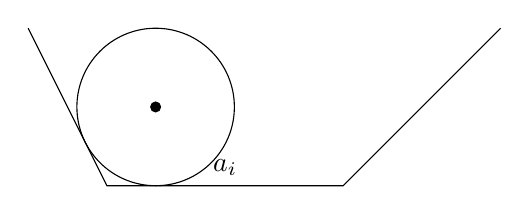
\begin{tikzpicture}
    \draw (0,2) -- (1,0) coordinate (a)
    -- (4,0) coordinate (b)
    -- (6,2);
    \draw (2.5,0) node[anchor=south] {$a_i$};
    % is this the golden ratio?
    \draw (1.618,1) circle (1cm);
    \fill (1.618,1) circle (2pt);
\end{tikzpicture}